\documentclass[%
  reprint,
  superscriptaddress,
  showpacs,
  showkeys,
  amsmath,amssymb,
  pra,
  longbibliography,
  floatfix,
  x11names
]{revtex4-2}

\usepackage{amsmath}
\usepackage{amssymb}
\usepackage{amsthm}
\usepackage{bm} % bold math
\usepackage{graphicx}
%\usepackage{times}
%\usepackage{mathptm}
\usepackage{tikz}
\usetikzlibrary{decorations.markings,lindenmayersystems}
\usepackage{pgfplots}
\pgfplotsset{compat=1.18}
\usepackage{orcidlink}
\usepackage{hyperref}

%
% --- DEFINITIONS FOR FIGURES (MUST BE IN PREAMBLE) ---
%

% Configuration parameters for Menger Sponge
\definecolor{cubeface1}{RGB}{180,180,180}  % Right face
\definecolor{cubeface2}{RGB}{220,220,220}  % Top face
\definecolor{cubeface3}{RGB}{140,140,140}  % Front face
\definecolor{cubeedge}{RGB}{80,80,80}      % Edge color

\newcommand\mengersponge[2][]{
    % Optional parameters: #1 = options, #2 = level
    \pgfkeys{
        /menger/.cd,
        draw edges/.initial=true,
        edge width/.initial=0.1pt,
        .unknown/.style={\pgfkeyscurrentname/.style={#1}}
    }
    \pgfkeys{/menger/.cd, #1}

    \pgfmathsetmacro\level{int(#2 - 1)}
    \ifnum \level = 0 \relax
        % Base case: draw a single cube with three visible faces
        \mengercube
    \else
        % Recursive case: draw 20 smaller cubes (3^3 - 7 holes)
        \begin{scope}[scale=0.333333]
            \foreach \x in {-2,0,2} {
                \foreach \y in {-2,0,2} {
                    \foreach \z in {-2,0,2} {
                        % Skip the 7 positions that create the characteristic holes
                        \pgfmathsetmacro{\skipthis}{
                            (\x==0 && \y==0) || (\x==0 && \z==0) || (\y==0 && \z==0) ? 1 : 0
                        }
                        \ifnum\skipthis=0
                            \begin{scope}[shift={(\x,\y,\z)}]
                                \mengersponge[#1]{\level}
                            \end{scope}
                        \fi
                    }
                }
            }
        \end{scope}
    \fi
}

\newcommand\mengercube{
    % Draw the three visible faces of a unit cube
    % Right face (x=1)
    \filldraw[
        fill=cubeface1,
        draw=cubeedge,
        line width=\pgfkeysvalueof{/menger/edge width}
    ] (1,1,1) -- (1,1,-1) -- (1,-1,-1) -- (1,-1,1) -- cycle;

    % Top face (y=1)
    \filldraw[
        fill=cubeface2,
        draw=cubeedge,
        line width=\pgfkeysvalueof{/menger/edge width}
    ] (1,1,1) -- (1,1,-1) -- (-1,1,-1) -- (-1,1,1) -- cycle;

    % Front face (z=1)
    \filldraw[
        fill=cubeface3,
        draw=cubeedge,
        line width=\pgfkeysvalueof{/menger/edge width}
    ] (1,1,1) -- (1,-1,1) -- (-1,-1,1) -- (-1,1,1) -- cycle;
}


% Define the Koch curve Lindenmayer system
\pgfdeclarelindenmayersystem{Koch curve}{
  \rule{F -> F+F--F+F}
}

% Define the Lindenmayer system rules for generating the Cantor set
\pgfdeclarelindenmayersystem{Cantor set}{
  \rule{F -> FfF}  % A line segment (F) is replaced by a segment, a gap, and another segment.
  \rule{f -> fff}  % A gap (f) is replaced by three gaps to maintain the correct scaling.
}
% --- END OF FIGURE DEFINITIONS ---
%



\begin{document}

\title{Anti-Gravity from Vacancies in Fractal Space-Time: The Case of a Menger Sponge}

\author{Karl Svozil\,\orcidlink{0000-0001-6554-2802}}
\email{karl.svozil@tuwien.ac.at}
\homepage{http://tph.tuwien.ac.at/~svozil}
\affiliation{Institute for Theoretical Physics, TU Wien, Wiedner Hauptstrasse 8-10/136, 1040 Vienna, Austria}

\date{\today}

\begin{abstract}
We propose that anti-gravity, interpreted as matter-matter repulsion, may emerge naturally in a fractal framework of spacetime characterized by vacancies (thinning out) rather than added matter. Using the Menger Sponge as a prototype, we construct an effective negative-mass Schwarzschild-like metric for embedded observers and compute the resulting curvature. We interpret the metric to derive the conditions for local repulsion. We also discuss the associated energy-condition violations, stability issues, and testable predictions.
\end{abstract}

\keywords{fractal gravity, anti-gravity, Menger sponge, embedded observers}

\maketitle

\section{Introduction}
\label{sec:intro}

How would an embedded observer~\cite{toffoli:79,svozil-94} experience~\cite{sv1} motion in a fractal~\cite{falconer1} substratum~\cite{Ord-83}? Throughout, ``embedded'' means an observer who has no kinematic access to any external Euclidean background.

The distinction between intrinsic and extrinsic perspectives is powerfully elucidated in Einstein's ``aether'' metaphor from his 1920 Leiden address~\cite{einstein-aether-en}. He used this analogy to differentiate his concept of a ``gravitational aether'' in general relativity from the discarded notion of a mechanical, light-carrying medium.

Einstein invites us to consider the surface of water upon which waves propagate, and the two vastly different conceptual models or ``mental images''~\cite{hertz-94e} one can construct. First, an extrinsic observer, viewing the system from outside, could track the motion of the underlying substance by tossing small corks onto the water. By following these markers, such an observer gains insight into the movements of the individual particles that constitute the medium.

In contrast, an intrinsic, embedded observer---a ``Flatlander''~\cite{abbott-flatland} confined to the two-dimensional water-air interface---lacks this external vantage point. Bound by their environment, they can only describe the evolving geometric shape of the waves. They perceive the patterns but have no direct access to the substance that supports them.

Einstein's critical insight emerges from a thought experiment: What if there were no ``corks,'' or more precisely, what if---even with the fluid present---no operational means existed to track its individual components? If the only observable phenomenon were the wave's changing form, one would have no grounds to assume the water consists of discrete, movable particles. Even so, Einstein argues, it could still rightfully be called a ``medium.''

This is precisely his reimagined aether: a geometric, gravitational fabric of spacetime that serves as a medium for light and matter, but whose constituent parts---if they exist---cannot be tracked. It represents a ``geometrized'' conception of a medium, devoid of ponderable, mechanical properties from the intrinsic viewpoint.

A modern parallel appears in phenomena like light bulbs or video playback. For an intrinsic observer unable to resolve events faster than the flicker fusion threshold (roughly 50--60 Hz), a discrete sequence of still frames manifests as perfectly continuous motion.

However, the conceptual models and Hertz's ``mental images''~\cite{hertz-94e} we adopt are far from trivial; they fundamentally shape the trajectory of scientific inquiry. To advance our understanding of spacetime, we must interrogate whether its apparent continuity is truly fundamental or merely an emergent property, much like the seamless flow of a video. Progress in physics may stall if we idealize the vacuum as an imponderable continuum, overlooking the possibility that it is, at a deeper level, composed of ``ponderable,'' tangible constituents. Acknowledging this potential could prove essential for unlocking pathways to a more complete theory of spacetime.

We speculate that ``thinning out'' spacetime leads to an intrinsic perception of negative curvature, manifesting as anti-gravity (repulsion) for observers within the structure. This contrasts with positive curvature from added matter, akin to defects in solids~\cite{Kroner-1958,kroner-1990}. Unlike particle-based interactions, this is a geometric effect, preserving the equivalence principle.

We build on relativity's geometric ether~\cite{einstein-aether-en,dirac-aether} and induced gravity from quantum fluctuations, as proposed by Sakharov~\cite{Sakharov-67}. Section~\ref{sec:intuitive} provides intuitive analogies, Section~\ref{sec:quant} presents a semi-quantitative analysis with explicit computations, Section~\ref{sec:geodesic} provides a direct test of repulsion via geodesic acceleration, Section~\ref{sec:energy} analyzes the energy conditions required for such a source, and Section~\ref{sec:discuss} discusses implications and predictions.

\section{Intuitive Analogies}
\label{sec:intuitive}

\subsection{Fractals and Embedded Observers}
The Menger Sponge, generated by iteratively starting with a unit cube and removing the central 1/9 from each face and the central cube, has a Hausdorff dimension of  $\log 20 /\log 3 \approx 2.7268$ and approaches a state where ``almost all'' volume is vacant in the limit.
As will be argued later, the effective dimension less than three implies a ``volume deficit'', which embedded observers perceive as shorter geodesics.
The third iteration is depicted in Fig.~\ref{fig:menger}. It is path-connected but riddled with vacancies, raising questions about continuous motion for intrinsic observers. This echoes Zeno's arrow paradox: apparent continuity may arise from momentum information, not spatial discreteness alone.

Operational metrics on fractals~\cite{Hodel-74,nagata_1985} involve geodesic distances $d_F(p,q)$, the shortest path length in the fractal set $F$~\cite{kigami-2020,gu-2023}. For embedded observers, these are measured by ``counting steps'' in the substratum~\cite{kroner-1985}, projecting fractal geometry onto effective continua~\cite{sv4}.

\begin{figure}[ht]
\centering
\resizebox{.36\textwidth}{!}{
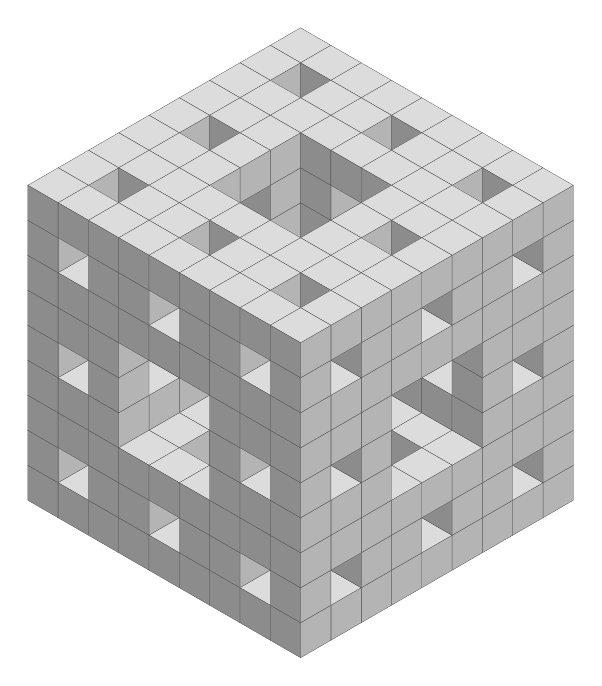
\begin{tikzpicture}[
    x={(0.866cm,-0.5cm)},
    y={(0cm,1cm)},
    z={(-0.866cm,-0.5cm)},
    scale=2
]
    \mengersponge{3}
\end{tikzpicture}
}
\caption{The Menger Sponge at resolution level  three (gray: material, transparent: vacancy).}
\label{fig:menger}
\end{figure}

\begin{figure}[ht]
\centering
\resizebox{0.36\textwidth}{!}{
  \begin{tikzpicture}
    \def\n{3} % Iteration level
    \draw[l-system={Koch curve, axiom=F, order=\n, angle=60, step=0.5cm}] lindenmayer system;
  \end{tikzpicture}
}
\caption{Extended line: Koch Curve at resolution level three.}
\label{fig:Koch}
\end{figure}


\begin{figure}[ht]
\centering
\resizebox{0.4\textwidth}{!}{
  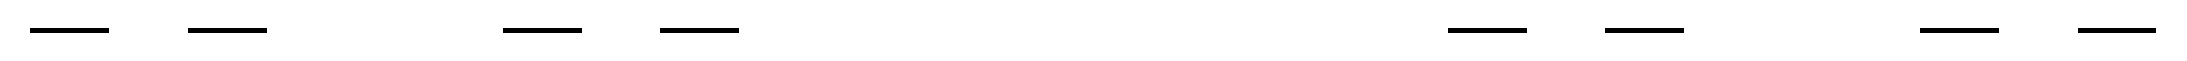
\begin{tikzpicture}
    \def\n{3} % Iteration level
    \draw[
      black,
      line width=2pt,
      l-system={
        Cantor set,
        axiom=F,
        order=\n,
        step=1cm
      }
    ]
    lindenmayer system;
  \end{tikzpicture}
}
\caption{Carved out line:  The Cantor Set at resolution level three.}
\label{fig:Cantor}
\end{figure}


\subsection{Analogy to Defects in Solids}
Relativity redefined the ether as geometric, not mechanical~\cite{einstein-aether-en}. Quantum fluctuations add ``ponderability'' (e.g., Casimir forces~\cite{Casimir_1948}), and Sakharov viewed gravity as emergent from vacuum elasticity~\cite{Sakharov-67}.

From the onset, the elasticity theory of solids has been linked to the formalism of the general theory of relativity~\cite{schaefer-1953,zaanen-2022}.
A geometrical approach to the theory of structural defects in solids by (four-dimensional)
continuum mechanics~\cite{Kroner-1958,kroner-1959,Kosevich-1962,Turski-66,kroner-1967,kroner-1975,Kossecka_deWit-77,kroner-1985,kroner-1990,kroner-2001,amari-1968,gunther-1972,Guenther-1979,gunther-1981,gunther-1983,golebiewska-lasota-1979a,golebiewska-lasota-1979b}
effectively~\cite{anderson:73} encodes defects in terms of  elastoplasticity.
This formalism is tensor based.

Already Kr\"oner emphasized the
operational, intrinsic viewpoint of embedded observers as being pertinent and fundamental~\cite{kroner-1990}:
``Imagine some crystal being who has just the ability to recognize
crystallographic directions and to count lattice steps along them. Such an
internal observer will not realize deformations from outside, and therefore
will be in a situation analogous to that of the physicist exploring the world.
This physicist clearly has the status of an internal observer.''
Therefore~\cite{kroner-1985}, ``lengths are measured and atoms identified by
counting lattice steps in the three crystallographic directions, then applying Pythagoras' theorem
$
ds^2 = g_{kl}\, dx^k dx^l,
$
where $ds$ is the distance of two atoms with relative position $dx^k$.
$\ldots$
$ds$ $\ldots$ is not the distance obtained by
an external observer by means of a constant scale, but is, rather, the distance found
by an internal observer with the help of the counting procedure''.

The aforementioned analogy between general relativity and the elasticity theory of solids
has led to speculations that dark matter is a solid~\cite{Bucher-PhysRevD.60.043505}.
Kleinert even speculated that a general relativity-type ``crystal gravity'' can be derived for a ``world crystal'' with defects~\cite{kleinert-1987,kleinert-2000,kroner-2001,kleinert-2004}.
In this analogy, the conserved defect tensor can be identified with the Einstein curvature tensor.
The fourth (time) dimension enters because of the dynamics: the movement of defects and the change of the crystal's plastic state~\cite{amari-1968}.

This can be intuitively understood~\cite{zaanen-2022} by the following mental image~\cite{hertz-94e} or metaphor:
Suppose you want to envelope a cone with a sheet of paper.
Due to the stiffness of the paper and its nonelasticity this will not be possible.
However, if you allow \emph{adding} stuff (that is, additional paper) to the paper (by cutting and gluing) you can
produce a paper that envelops any kind of surface, including the cone. As a consequence of akignment such an envelope will bow out of the originally flat
paper plane, and produce a non-flat curvature.

This additional stuff will also produce  ``longer paths'' from one end of the paper to another,
as crossing over or around the envelope of the cone requires more steps (from ``added stuff'') than on the originally flat surface.
A typical example of such a situation is the Koch Curve depicted in Fig.~\ref{fig:Koch}.
Therefore, relative to ``free space'' without defects, adding material (disclination) lengthens geodesics.
Intrinsically, this will be experienced as the tendency of bodies to ``delay separation'' and ``stay together'', thus mimicking attraction.

Conversely, \emph{removing} stuff (vacancies) creates ``shortcuts,'' the capacity to cross points in space
along a ``shorter path''. This will be intrinsically experienced not as contraction but as an expansion,
such that bodies move away from each other faster, suggesting repulsion.
A canonical example of such a cut-out configuration is the Cantor Set, depicted in Fig.~\ref{fig:Cantor}.
Likewise, for Menger Sponge observers, vacancies reduce traversable material, accelerating motion intrinsically---perceived as anti-gravity.
%This mirrors how positive Ricci curvature in general relativity causes geodesic convergence (attraction), while negative causes divergence (repulsion).

\section{Semi-Quantitative Analysis}
\label{sec:quant}

\subsection{Motivation from the Schwarzschild Metric}

To construct a physically robust model for a localized defect, we move away from analogies based on elastic media and instead draw inspiration from the foundational solution of General Relativity: the Schwarzschild metric. This metric provides the exact description of the spacetime geometry outside a static, spherically symmetric point mass, $M$. It is the blueprint for any localized, static gravitational source.

The Schwarzschild metric is given by:
\begin{equation}
g_{\mu\nu} = \text{diag}\left[-\left(1 - \frac{2M}{r}\right), \left(1 - \frac{2M}{r}\right)^{-1}, r^2, r^2 \sin^2 \theta\right]
\label{eq:schwarzschild}
\end{equation}
The term $2M/r$ dictates the gravitational interaction. Because $M$ is a positive mass, this term leads to the attractive force we call gravity.

Our central hypothesis is to model the effect of a crystalline defect in an analogous manner. We propose that the net density of defects acts as a form of ``gravitational charge'', replacing the mass $M$ as the source of spacetime curvature. The sign of this net charge should determine whether the interaction is attractive or repulsive.

\subsection{Derivation of the Defect-Induced Metric}

\subsubsection{Defining the Gravitational Source Term}

We define the net defect strength, $S$, as the difference between the interstitial density ($N_i$) and the vacancy density ($N_v$):
\begin{equation}
S = N_i - N_v
\end{equation}
This dimensionless quantity represents our ``gravitational charge''. If interstitials dominate ($S>0$), we expect one behavior; if vacancies dominate ($S<0$), we expect the opposite.

To connect this to the fractal structure of the Menger Sponge, we derive an effective form for the source term. At iteration level $n$, the Sponge retains a volume fraction of $(20/27)^n$ of the original unit cube, implying a vacancy fraction
\begin{equation}
v = 1 - (20/27)^n.
\end{equation}
For a vacancy-dominated case (as in our model), we set $S = -v$ (with $N_i \approx 0$), capturing the ``thinning out'' effect. The fundamental length scale $L$ is taken as the initial lattice spacing (e.g., the side length of the starting cube, with units of length). The product $S \cdot L = -v L$ then represents an effective ``negative gravitational radius'', scaling the metric perturbation based on the fractal vacancies.

A direct substitution of $M \to S$ in Equation~\ref{eq:schwarzschild} is, however, dimensionally inconsistent and not rigorously derived. In geometrized units (where $G=c=1$), the mass $M$ has units of length, whereas our strength $S$ is dimensionless. Note that $L$ has units of [length], $S$ is dimensionless, so $S L$ has units of [length] like $M$. We therefore perform an analogous substitution $2M \longrightarrow S \cdot L$, treating the net defect strength as an effective gravitational source inspired by the fractal vacancy structure. The term $S \cdot L$ is now a length, just like $2M$, and can be interpreted as the ``effective gravitational radius'' of the net defect. Since $0 \le N_i, N_v \le 1$, this ``effective mass'' term $S \cdot L$ is no longer positive definite: indeed, for vacancies in a medium, $N_i=0$ and $N_v > 0$, and we thus get a negative effective mass~\cite{bondi-1957}.

\subsubsection{The General Metric for a Localized Defect}
\label{2025-menger-gmld}
By performing this substitution in the Schwarzschild blueprint~(\ref{eq:schwarzschild}), we arrive at a general metric that describes the spacetime around a localized defect concentration:
\begin{equation}
g_{\mu\nu} = \text{diag}\left[-\left(1 - \frac{S \cdot L}{r}\right), \left(1 - \frac{S \cdot L}{r}\right)^{-1}, r^2, r^2 \sin^2 \theta\right]
\label{eq:defect_metric}
\end{equation}
This metric now provides a unified framework whose physical interpretation depends entirely on the sign of the net defect strength, $S$.

\subsection{Analysis of Physical Regimes}

\subsubsection{The Attractive Regime: Interstitial Domination ($N_i > N_v$)}

In the case where the density of interstitials is greater than that of vacancies, the net defect strength $S$ is positive.
\begin{itemize}
    \item The metric takes the exact mathematical form of the standard Schwarzschild metric for a positive mass.
    \item The ``slope of time'' is negative ($\partial_r g_{tt} < 0$), creating a ``time valley''.
    \item {The resulting gravitational interaction is attractive.} Particles are pulled toward the defect.
    \item This spacetime possesses an event horizon at the radius $r_h = S \cdot L$.
\end{itemize}

\subsubsection{The Repulsive Regime: Vacancy Domination ($N_v > N_i$)}

In the case where the density of vacancies is greater than that of interstitials, the net defect strength $S$ is negative. Let us write $S = -|S|$. The time component of the metric becomes:
\begin{equation}
g_{tt} = -\left(1 - \frac{-|S| \cdot L}{r}\right) = -\left(1 + \frac{|S| \cdot L}{r}\right)
\end{equation}
The full metric is therefore:
\begin{equation}
g_{\mu\nu} = \text{diag}\left[-\left(1 + \frac{|S|L}{r}\right), \left(1 + \frac{|S|L}{r}\right)^{-1}, r^2, r^2 \sin^2 \theta\right]
\end{equation}
The properties of this spacetime are dramatically different:
\begin{itemize}
    \item The ``slope of time'' is positive ($\partial_r g_{tt} > 0$), creating a ``time hill''.
    \item The resulting gravitational interaction is repulsive. Particles are pushed away from the defect.
    \item This spacetime has {no event horizon}, as the condition $g_{tt}=0$ can never be satisfied for a positive radius $r$.
\end{itemize}
This model successfully describes a repulsive field, sourced by a net vacancy concentration,
that is valid for all radii outside the central singularity.
This is consistent with Bondi's analysis of negative masses in general relativity~\cite{bondi-1957}.

\section{Analysis of the Ricci Scalar}
\label{sec:ricci}

The Ricci scalar, $R$, is a fundamental invariant in Riemannian geometry that measures the intrinsic curvature of spacetime at a point. Its physical significance is made clear through the trace of the Einstein field equations in geometrized units (assuming no cosmological constant, $\Lambda=0$):
\begin{equation}
    R = -8\pi T,
\end{equation}
where $T = T^\mu{}_\mu$ is the trace of the stress-energy tensor, representing the sum of energy density and pressures. Calculating the Ricci scalar for our proposed metric therefore allows us to determine the physical nature of the spacetime it describes. From this relation, $R=0$ implies $T=0$, confirming that the spacetime is a vacuum outside the central defect, with curvature sourced solely by the singularity at $r=0$.

\subsection{Calculation for the Defect Metric}

The metric~(\ref{eq:defect_metric}) for the localized defect in Section~\ref{2025-menger-gmld}
has the   same mathematical form  as the Schwarzschild metric, with the term $2M$ simply replaced by the constant parameter $S \cdot L$. We can therefore leverage the well-known properties of the Schwarzschild solution.

The Schwarzschild metric is, by its very definition, a {vacuum solution} to the Einstein Field Equations for all radii $r > 0$. This means it describes a region of spacetime devoid of matter and energy. The mathematical condition for a vacuum solution is that the entire Ricci tensor is zero:
\begin{equation}
    R_{\mu\nu} = 0 \text{ for } r > 0
\end{equation}
The Ricci scalar, $R$, is the trace of the Ricci tensor, defined as $R = g^{\mu\nu} R_{\mu\nu}$. Since every component of the Ricci tensor is zero, their trace must also be zero.

Therefore, without the need for a new, lengthy calculation, we can state with certainty that for our proposed metric, the Ricci scalar is:
\begin{equation}
     R = 0  \text{ for all } r > 0
\end{equation}
This holds true regardless of whether the metric is in its attractive ($S>0$) or repulsive ($S<0$) form.

\subsection{Physical Interpretation of a Vanishing Ricci Scalar}

The result $R=0$ might seem paradoxical. How can a spacetime that clearly produces a gravitational force (attraction or repulsion) have zero Ricci curvature?

This highlights a crucial distinction in General Relativity:
\begin{enumerate}
    \item {Ricci Curvature ($R_{\mu\nu}$):} This type of curvature is directly sourced by local matter and energy. The fact that $R_{\mu\nu}=0$ confirms that our metric correctly describes a spacetime that is a {vacuum} everywhere except for the origin. The trace relation $R = -8\pi T$ confirms this, as $R=0$ implies $T=0$.

    \item {Weyl Curvature (Tidal Forces):} The full curvature of spacetime is described by the more general Riemann curvature tensor, $R^\rho{}_{\sigma\mu\nu}$. Even when the Ricci tensor is zero, the Riemann tensor can be non-zero. This remaining part of the curvature is called the Weyl curvature, and it is responsible for the tidal forces and the gravitational field in a vacuum.
\end{enumerate}

In essence, a vanishing Ricci scalar does not mean ``no curvature'' or ``no gravity''. It means that the gravitational field is being sourced by a central object (a singularity at $r=0$) and is propagating through empty space. The curvature exists in the form of tidal forces that would stretch or squeeze an object, which is precisely what causes geodesic deviation---the phenomenon we perceive as a gravitational force.

Therefore, the result $R=0$ serves as a powerful consistency check, confirming that our model correctly describes a localized point-like source whose gravitational influence extends into an otherwise empty spacetime.

\section{Detailed Analysis via Geodesic Motion}
\label{sec:geodesic}

While the Ricci scalar confirms that our spacetime is a vacuum solution, it does not directly reveal the attractive or repulsive nature of the gravitational field. To analyze the force experienced by test particles, we must turn to the equations that govern their motion. The most fundamental of these is the geodesic equation, whose consequences are elegantly summarized by the Raychaudhuri equation.

We will first use the geodesic equation to directly calculate the initial acceleration of a stationary particle. This provides the definitive physical answer. We will then use this result to understand the behavior of the Raychaudhuri equation in this context.

\subsection{The Direct Physical Test: Geodesic Acceleration}

The most intuitive way to determine if a field is attractive or repulsive is to place a test particle at rest and see which way it begins to move. In General Relativity, this initial acceleration is governed by the geodesic equation, $a^\mu = -\Gamma^\mu_{\nu\lambda}u^\nu u^\lambda$.

\subsubsection{Setup}
Consider an observer at a fixed position $(r, \theta, \phi)$. For this observer to be at rest, their only motion is through time. Their four-velocity is $u^\mu = (u^t, 0, 0, 0)$. Due to the normalization condition $g_{\mu\nu}u^\mu u^\nu = -1$, we have $g_{tt}(u^t)^2 = -1$.

The radial component of the particle's acceleration is given by:
\begin{equation}
a^r = -\Gamma^r_{tt} (u^t)^2 = -\Gamma^r_{tt} \left(\frac{-1}{g_{tt}}\right) = \frac{\Gamma^r_{tt}}{g_{tt}}
\end{equation}
The sign of this acceleration will tell us the direction of the force.

\subsubsection{Calculation}
We need to compute the Christoffel symbol $\Gamma^r_{tt}$ for our general metric, where $g_{tt} = -(1 - SL/r)$.
\begin{equation}
\Gamma^r_{tt} = -\frac{1}{2} g^{rr} \frac{\partial g_{tt}}{\partial r}
\end{equation}
First, we find the components:
\begin{align*}
\frac{\partial g_{tt}}{\partial r} &= \frac{\partial}{\partial r}\left(-1 + \frac{SL}{r}\right) = -\frac{SL}{r^2} \\
g^{rr} &= \frac{1}{g_{rr}} = 1 - \frac{SL}{r}
\end{align*}
Now, we assemble the Christoffel symbol:
\begin{equation}
\Gamma^r_{tt} = -\frac{1}{2} \left(1 - \frac{SL}{r}\right) \left(-\frac{SL}{r^2}\right) = \frac{SL}{2r^2}\left(1 - \frac{SL}{r}\right)
\end{equation}
Finally, we calculate the radial acceleration $a^r$:
\begin{equation}
a^r = \frac{\Gamma^r_{tt}}{g_{tt}} = \frac{\frac{SL}{2r^2}\left(1 - \frac{SL}{r}\right)}{-\left(1 - \frac{SL}{r}\right)} = -\frac{SL}{2r^2}
\end{equation}
This is our definitive result for the initial acceleration of a stationary particle upon release.

\subsubsection{Analysis of Results}
Let's analyze the sign of $a^r = -SL/(2r^2)$ in our two physical regimes.
\begin{itemize}
    \item {Attractive Case ($N_i > N_v$ implies $S > 0$):}
    The acceleration is $a^r = -|S|L/(2r^2)$, which is {negative}. A negative radial acceleration means the particle moves toward the origin. This confirms the force is attractive.

    \item {Repulsive Case ($N_v > N_i$ implies $S < 0$):}
    The acceleration is $a^r = -(-|S|)L/(2r^2) = +|S|L/(2r^2)$, which is {positive}. A positive radial acceleration means the particle moves away from the origin. This confirms the force is repulsive.
\end{itemize}
The geodesic equation thus gives an unambiguous answer that matches our physical intuition.

\subsection{The Raychaudhuri Equation and the Curvature Paradox}

How does the direct calculation of acceleration relate to the Raychaudhuri equation? The equation describes the evolution of the expansion scalar $\theta$ for a geodesic congruence, representing the volume change of a cloud of free-falling particles. For an initially static, non-rotating congruence ($\theta=0$, $\omega=0$), it simplifies to
\begin{equation}
\frac{d\theta}{d\tau} = - \sigma_{\mu\nu}\sigma^{\mu\nu} - R_{\mu\nu}u^\mu u^\nu,
\label{eq:raychaudhuri}
\end{equation}
where $\sigma_{\mu\nu}$ is the shear tensor (measuring tidal distortion).

Here we encounter an apparent paradox. We established that for our metric, the Ricci tensor $R_{\mu\nu}$ is zero everywhere (for $r>0$). This would seem to simplify the equation to:
\begin{equation}
\frac{d\theta}{d\tau} = - \sigma^2 \quad (\textit{Apparent Result}).
\end{equation}
Since the shear-squared term $\sigma^2$ is always non-negative, this would imply that $d\theta/d\tau$ is always negative or zero. A negative $d\theta/d\tau$ signifies contraction, meaning attraction. This seems to contradict our finding that repulsion is possible.

The resolution lies in the full geodesic deviation equation, $D^2 \xi^\mu / D\tau^2 = - R^\mu{}_{\nu\rho\sigma} u^\nu \xi^\rho u^\sigma$, from which the Raychaudhuri equation is derived, showing that the relative acceleration between particles depends directly on the full Riemann tensor $R^\rho{}_{\sigma\mu\nu}$. While the Ricci tensor (a trace of the Riemann tensor) is zero in a vacuum, the Riemann tensor itself is not: Its components cause tidal forces and are proportional to $S L$ (or M).

For $S<0$, the sign flip reverses tidal forces, causing defocusing despite the scalar Raychaudhuri form. The shear $\sigma$ is induced by Weyl curvature, and its evolution (governed by Weyl terms with sign of $S$) leads to net expansion for negative $S$. A detailed calculation in Appendix~\ref{app:shear} shows that the magnitude $\sigma^2$ depends on the square of the Riemann tensor components, but the scalar Raychaudhuri equation is a trace, and some information is lost: Repulsion is encoded in the tensor structure. Thus, while the vacuum saturates the Strong Energy Condition ($R_{\mu\nu} u^\mu u^\nu =0$), the source at $r=0$ effectively violates it for repulsion.

The clearest picture comes from the geodesic equation itself. The non-zero acceleration $a^r = -SL/(2r^2)$ is the direct physical manifestation of the underlying curvature described by the full Riemann tensor. The sign of $S$ dictates the sign of the curvature, which in turn dictates the sign of the acceleration, and this is what determines if a cloud of released particles will begin to expand (repulsion) or contract (attraction).

\section{Energy Condition Remarks}
\label{sec:energy}

Energy conditions are a set of criteria in General Relativity used to constrain the stress-energy tensor ($T_{\mu\nu}$). They represent fundamental assumptions about the nature of matter and energy, essentially separating ``physically reasonable'' matter from ``exotic matter''. Analyzing these conditions for our derived metric is crucial for understanding the physical nature of the defect source, particularly in the case of repulsion.

\subsection{Analysis in the Vacuum ($r > 0$)}

As established, our metric is a vacuum solution to the Einstein Field Equations for all radii outside the origin ($r>0$). This means the stress-energy tensor is identically zero in this region:
\begin{equation}
    T_{\mu\nu} = 0 \text{ for } r > 0
\end{equation}
As such, all standard energy conditions, which are inequalities involving $T_{\mu\nu}$, are trivially satisfied in this vacuum region. For example, the Null Energy Condition (NEC), which states that $T_{\mu\nu}k^\mu k^\nu \ge 0$ for any null vector $k^\mu$, becomes $0 \ge 0$. This holds true.

The important conclusion is that the vacuum spacetime itself is not composed of exotic matter. The source of the gravitational field must therefore be entirely confined to the point at the origin.

\subsection{The Strong Energy Condition and the Nature of Gravity}

The Strong Energy Condition (SEC) is the most relevant for discussing gravitational attraction. Through the Einstein equations, the SEC can be stated as a purely geometric condition:
\begin{equation}
    R_{\mu\nu}u^\mu u^\nu \ge 0
\end{equation}
for any timelike vector $u^\mu$. The Raychaudhuri equation shows that this condition guarantees that gravity is attractive (or at worst, non-repulsive). Gravitational repulsion requires a violation of the SEC.

In our analysis of the Ricci scalar, we found that for our metric, the Ricci tensor is zero everywhere ($R_{\mu\nu}=0$) outside the origin. Therefore, our solution satisfies:
\begin{equation}
    R_{\mu\nu}u^\mu u^\nu = 0
\end{equation}
This means our spacetime {saturates the Strong Energy Condition}. It sits on the precise boundary between attraction and repulsion. The vacuum itself does not ``lean'' one way or the other. This reinforces the conclusion that the character of the force must originate entirely from the nature of the singularity at $r=0$.

\subsection{Implications for the Source at the Origin}

The true physical nature of the defect is revealed by considering what kind of source at $r=0$ is required to produce the surrounding geometry. The ``effective gravitational mass'' of the source is proportional to our strength term, $S = N_i - N_v$.

\begin{itemize}
    \item {Attractive Case ($S > 0$):}
    When interstitials dominate, the source has a positive effective gravitational mass. The singularity at $r=0$ behaves like normal matter concentrated at a point. It satisfies the energy conditions in an averaged sense, consistent with our everyday experience of gravity.

    \item {Repulsive Case ($S < 0$):}
    When vacancies dominate, the source must have a negative effective gravitational mass. This is the hallmark of  exotic matter. For the singularity at $r=0$ to generate a repulsive field, it must be composed of matter that violates the standard energy conditions. This could be interpreted as a region of immense negative pressure or tension, so large that it overcomes its own energy density to produce a net repulsive gravitational effect.
\end{itemize}

In summary, while the spacetime for $r>0$ is a vacuum that satisfies all energy conditions, the character of the central singularity is fundamentally different in the two regimes. The attractive case can be sourced by conventional matter, but the repulsive case necessitates that the origin is a source of exotic matter. This provides a complete and self-consistent physical picture that connects the microscopic details of the defect ($N_i$ vs. $N_v$) to the macroscopic laws of General Relativity.

A notational remark seems in order:
Throughout the paper we keep the product $SL$ itself as the source parameter.
If one rewrites the line element in the textbook Schwarzschild form
$ds^{2} \;=\;
- \left(1-\frac{2M}{r}\right) dt^{2}
\;+\;
\left(1-\frac{2M}{r}\right)^{-1} dr^{2}
\;+\;
r^{2} d\Omega^{2}$,
one identifies
$
2M = SL$ with $\quad M=\tfrac12 SL $.

\section{Discussion}
\label{sec:discuss}

This approach reconceptualizes curvature, linking it specifically to fractal dimensionality and, more broadly, to the density of spacetime.
Based on this principle, this work has established a geometric framework for anti-gravity arising from fractal spacetime vacancies,
demonstrating that repulsive gravitational effects emerge naturally when spacetime exhibits a fractal structure characterized by systematic removal of volume. By employing the Menger Sponge as a prototypical fractal, we derived an effective metric for embedded observers and analyzed the conditions for repulsion. Our analysis reveals that the defect-induced metric~(\ref{eq:defect_metric}) provides a unified description of both attractive and repulsive regimes, with the sign of the net defect strength $S = N_i - N_v$ determining the nature of the gravitational interaction.

Mathematically, we essentially present a re-interpretation of the negative-mass Schwarzschild solution.
The innovation is the fractal interpretation;
a reconceptualization of (anti-)gravity as an intrinsic geometric property of spacetime topology rather than an exotic particle interaction.
This perspective aligns with Sakharov's vision of gravity emerging from vacuum fluctuations while extending it to fractal geometries.
The solid-defect analogy---where vacancies create ``shortcuts'' that manifest as repulsion---offers an intuitive bridge between condensed matter physics and general relativity. Crucially, this model preserves the equivalence principle, as repulsion arises from the observer's intrinsic experience of fractal geometry, not external forces. The geodesic analysis confirms that test particles experience outward acceleration $a_r = -\frac{S \cdot L}{2r^2}$ when $S < 0$, directly satisfying the condition for matter-matter repulsion. Meanwhile, the energy condition analysis reveals that while the vacuum exterior ($r > 0$) trivially satisfies all energy conditions, the origin ($r = 0$) requires exotic matter with negative effective mass to sustain repulsion, highlighting a fundamental distinction between geometric vacancies and conventional matter.

One might be tempted to identify the source for negative effective mass as some form of quantum field theoretic consequence~\cite{kontou-2020},
like the Casimir effect~\cite{bekenstein-2013,costa-2022}.
However, such an approach should be considered unsettled at best~\cite{Santiago22-PhysRevD.105.064038}.

Despite its mathematical rigor, the model faces significant physical and conceptual challenges.
The empirical justification for fractal spacetime remains a primary concern, as the Menger Sponge structure,
while mathematically elegant, lacks observational support.
Quantum gravity scales (e.g., Planck length) may invalidate classical fractal descriptions.
Additionally, the repulsive regime necessitates a point-like exotic source at $r = 0$,
raising unresolved questions about stability, quantum consistency, and physical realizability:
Negative mass implies run-away instabilities~\cite{bondi-1957}.
While we allude to testable predictions, concrete observables remain undeveloped.
Furthermore, the solid-defect model may break down at cosmological scales or in strong-field regimes where torsion or quantum effects dominate.

To advance this framework, several promising directions warrant exploration.
Incorporating fractal vacancies into quantum gravity models through path integrals
over fractal geometries could resolve the singularity and explore Planck-scale effects.
Investigating whether fractal vacancies contribute to dark energy presents another compelling avenue,
as their repulsive nature mimics cosmic acceleration.
Deriving precise predictions for light propagation delays in fractal regions,
anomalous perihelion precession in repulsive fields (e.g., negative gravitational lensing with defocusing of light rays and anomalous orbital decay in fractal regions),
and gravitational wave echoes from fractal-induced metric perturbations would enhance empirical testability.
Extending the analysis to other fractals (e.g., Sierpinski carpets) could identify universal features of vacancy-driven repulsion.
Finally, examining the stability of repulsive solutions against perturbations, particularly in the context of energy-condition violations, remains essential.

This work establishes fractal spacetime vacancies as a viable mechanism for anti-gravity,
offering a geometric alternative to particle-based explanations.
 While the model is mathematically self-consistent and conceptually compelling,
its physical relevance hinges on future empirical validation and quantum refinement.
Should fractal structures emerge in quantum gravity or cosmological observations,
vacancy-induced repulsion could provide a unified explanation for phenomena ranging from dark energy to exotic compact objects.
Until then, this framework serves as a provocative invitation to reconceptualize gravity
through the lens of fractal geometry---where ``nothing'' (vacancies) and ``additions'' or ``accumulations'' (disclinations) may ultimately shape the dynamics of intrinsic spacetime.

\begin{acknowledgments}
This text was partially created and revised with assistance from one or more of the following large language models: Grok4-0709, Gemini 2.5 Pro, o3-2025-04-16, claude-sonnet-4-20250514-thinking-32k, GLM-4.5. All content, ideas, and prompts were provided by the author.
This research was funded in whole or in part by the  Austrian Science Fund (FWF) Grant DOI: 10.55776/PIN5424624.
The authors acknowledge TU Wien Bibliothek for financial support through its Open Access Funding Programme.
\end{acknowledgments}



\appendix

\section{Shear, Geodesic Deviation, and the Raychaudhuri Paradox}
\label{app:shear}

In this appendix, we provide a detailed calculation to resolve the apparent paradox in the Raychaudhuri equation for our defect-induced metric (Equation~\ref{eq:defect_metric}). The vacuum nature of the spacetime for $r > 0$ implies $R_{\mu\nu} = 0$. Consequently, the simplified Raychaudhuri equation, $d\theta/d\tau = -\sigma^2$, suggests that the expansion scalar $\theta$ can only be non-increasing ($\leq 0$), implying universal geodesic convergence (attraction). This contradicts our finding that for a negative defect strength $S<0$ (arising from fractal vacancies), geodesics diverge (repulsion).

We resolve this by examining the structure of the Weyl tensor, showing that repulsion is encoded in its tensor components (proportional to $S$), while the scalar $\sigma^2$ depends on their square, losing the sign. While the vacuum spacetime saturates the Strong Energy Condition (SEC, $R_{\mu\nu} u^\mu u^\nu = 0$), the source at $r=0$ must effectively violate it to produce a repulsive field.

\subsection{Geodesic Deviation and Tidal Forces}
The relative motion of nearby geodesics is described by the geodesic deviation equation for a connecting vector $\xi^\mu$:
\begin{equation}
\frac{D^2 \xi^\mu}{D\tau^2} = - R^\mu_{\ \nu\rho\sigma} u^\nu \xi^\rho u^\sigma = -K^\mu_{\ \rho} \xi^\rho,
\label{eq:geodev}
\end{equation}
where $u^\mu$ is the four-velocity of the central geodesic and $K^\mu_{\ \rho} = R^\mu_{\ \nu\rho\sigma} u^\nu u^\sigma$ is the tidal tensor. This equation describes how a cloud of test particles is tidally deformed by spacetime curvature. It is crucial to distinguish this relative acceleration (tidal forces) from the absolute acceleration of the entire cloud, which is governed by the geodesic equation itself ($a^\mu = -\Gamma^\mu_{\nu\lambda} u^\nu u^\lambda$), as computed in Section~\ref{sec:geodesic}.

\subsection{Curvature Components for the Defect Metric}
To compute these tidal effects, we evaluate the relevant curvature components. Our metric is isometric to the Schwarzschild metric with the substitution $2M \to \beta = SL$. As a vacuum solution, its curvature is entirely described by the Weyl tensor. For a congruence of observers at rest ($u^\mu = (u^t, 0, 0, 0)$), the tidal forces are described by the electric part of the Weyl tensor, $E_{\mu\nu} = R_{\mu\alpha\nu\beta}u^\alpha u^\beta$ (the trace-free tensor encoding tidal fields). We analyze its components in a local orthonormal frame $(\hat{t}, \hat{r}, \hat{\theta}, \hat{\phi})$ adapted to the spherical symmetry, where they are coordinate-independent and simplify calculations.

The non-zero components in this frame are:
\begin{align}
E_{\hat{r}\hat{r}} &= -\frac{\beta}{r^3}, \\
E_{\hat{\theta}\hat{\theta}} = E_{\hat{\phi}\hat{\phi}} &= \frac{\beta}{2r^3}.
\end{align}
The trace is manifestly zero ($E^\mu_{\ \mu} = E_{\hat{r}\hat{r}} + E_{\hat{\theta}\hat{\theta}} + E_{\hat{\phi}\hat{\phi}} = 0$), consistent with the vacuum condition $R_{\mu\nu}u^\mu u^\nu = 0$. Crucially, the sign of every component is determined by the sign of $\beta = SL$.

\begin{itemize}
    \item {Attractive case ($\beta > 0$):} $E_{\hat{r}\hat{r}} < 0$ causes particles separated radially to accelerate away from each other (stretching), while $E_{\hat{\theta}\hat{\theta}} > 0$ causes particles separated transversely to accelerate toward each other (squeezing). This tidal field focuses the congruence.
    \item {Repulsive case ($\beta < 0$):} All signs flip. $E_{\hat{r}\hat{r}} > 0$ causes radial squeezing (particles accelerate toward each other), while $E_{\hat{\theta}\hat{\theta}} < 0$ causes transverse stretching (particles accelerate away from each other). This ``anti-tidal'' force defocuses the congruence, causing net expansion.
\end{itemize}

\subsection{Shear Evolution and the Resolution}
The shear tensor, $\sigma_{\mu\nu}$, measures the rate of distortion of a congruence. For particles released from rest, the initial shear is zero ($\sigma_{\mu\nu}|_0 = 0$), but the tidal forces described by $E_{\mu\nu}$ will immediately induce shear. After a small proper time $\delta\tau$, the shear tensor will be approximately $\sigma_{\mu\nu} \approx E_{\mu\nu} \delta\tau$.

The shear-squared term in the Raychaudhuri equation is therefore:
\begin{align}
\sigma^2 = \sigma_{\mu\nu}\sigma^{\mu\nu} &\approx (E_{\mu\nu}E^{\mu\nu}) (\delta\tau)^2 \nonumber \\
&= \left[ (E_{\hat{r}\hat{r}})^2 + (E_{\hat{\theta}\hat{\theta}})^2 + (E_{\hat{\phi}\hat{\phi}})^2 \right] (\delta\tau)^2 \nonumber \\
&= \left[ \left(-\frac{\beta}{r^3}\right)^2 + 2\left(\frac{\beta}{2r^3}\right)^2 \right] (\delta\tau)^2 \nonumber \\
&= \left( \frac{\beta^2}{r^6} + \frac{\beta^2}{2r^6} \right) (\delta\tau)^2 = \frac{3}{2}\frac{\beta^2}{r^6}(\delta\tau)^2.
\end{align}
This result is the key to resolving the paradox. The term $\sigma^2$ is proportional to $\beta^2 = (SL)^2$ and is therefore \emph{always non-negative}, regardless of whether the field is attractive or repulsive. When the scalar Raychaudhuri equation is formed, the sign information contained in the individual components of the tidal tensor is lost. The equation $d\theta/d\tau = -\sigma^2$ correctly shows that induced shear always contributes negatively to the rate of change of volume, but it fails to capture the overall expansive or contractive nature of the tidal field itself, which is what truly determines repulsion or attraction. In the full, integrated Raychaudhuri dynamics, the sign of $\beta$ governs the evolution: for $\beta < 0$, the reversed tidal forces lead to net positive $d\theta/d\tau > 0$ (expansion) over time, despite the negative contribution from $-\sigma^2$.

\subsection{Implications for Energy Conditions}
In the vacuum region ($r > 0$), our metric satisfies $R_{\mu\nu} u^\mu u^\nu = 0$, meaning it \emph{saturates} the Strong Energy Condition. The vacuum itself is neutral. However, the global character of the spacetime (attractive or repulsive) is determined by the source at $r=0$. To generate the surrounding geometry, this source must have an effective mass proportional to $\beta$. For the repulsive case ($\beta < 0$), the source must be a singularity of negative effective mass, which violates the averaged Strong Energy Condition (requiring exotic matter with $T_{\mu\nu} u^\mu u^\nu < 0$ in an integrated sense). This violation is encoded in the structure of the full Riemann tensor, not the Ricci scalar or tensor, resolving the apparent paradox. In the context of fractal vacancies, such as the Menger Sponge, this negative effective mass arises from the geometric ``thinning out,'' providing a physical mechanism for intrinsic repulsion.


\bibliography{svozil}

\end{document}
